\section{Linear elasticity}

In this section, we study the simplest mathematical model for elastic
deformation of solids based on Hooke's law. For comparison,
consider~\cite{Braess97,Braess13}. For the full nonlinear model in all
mathematical detail refer to~\cite{Ciarlet88}.

\begin{Notation}{vector-diff-operators}
  Differential operators for vector fields $u:\R^d\to\R^d$
  are defined as follows:
  \begin{xalignat}2
    \nabla u &=
    \begin{pmatrix}
      \d_1 u_1 & \cdots & \d_d u_1\\
      \vdots && \vdots \\
      \d_1 u_d & \cdots & \d_d u_d
    \end{pmatrix}
    &&\text{(gradient)}
    \\
    \div u &= \sum_{i=1}^d \d_i u_i
    &&\text{(divergence)}
  \end{xalignat}

  For a tensor field $\sigma: \R^d\to \R^{d\times d}$, the divergence
  is a vector defined column-wise as
  \begin{gather}
    \div\sigma = \left(\sum_{i=1}^d \d_i \sigma_{ij}\right)_{j=1,\dots,d}
  \end{gather}
\end{Notation}

\begin{intro}
  The deformation of a solid body is described as a mapping $\Phi$
  from the \define{reference configuration} $\domain\subset \R^d$ to a
  deformed configuration $\deformed\domain \subset \R^d$, such that
  each undeformed point $x\in\domain$ is mapped to the point
  $\deformed x$ after deformation. The domain $d$ is 3 for physically
  relevant models, but we investigate two-dimensional problems in
  order to study mathematical properties and numerical methods more
  easily.

  Actually, we are not quite interested in this mapping $\Phi$, since
  it depends on the position of the points $x$. On the other hand, a
  basic principle of physical laws is frame invariance, namely, if we
  change from one Cartesian coordinate system to another, the physical
  law may only change by the same coordinate transformation, not in
  its physical implications. Therefore, only the differences
  $\deformed x-x$ should matter. Thus, we introduce the
  \define{displacement} $u$, such that
  \begin{gather*}
    \Phi = \id + u.
  \end{gather*}
  The symbol $\id$ will refer to all occurrences of identical mappings
  and their matrices.

  So far, by the introduction of $u$, we divide translations of the
  reference configuration out of our model. But, in addition, we have
  to eliminate the influence of solid body rotations. These are
  operations, which leave all distances and angles unchanged. Thus, we
  investigate the change of the distance between $x$ and $x+z$ under
  the mapping $\Phi$. By definition of the derivative, we have
  \begin{align*}
    \abs{\Phi(x+z) - \Phi(x)}^2 &= \norm{\nabla\Phi z} + o(\abs{z})
    \\
                              &= z^T\nabla\Phi^T\nabla\Phi z + o(\abs{z})
    \\
    &= z^T(I + \nabla u^T + \nabla u + \nabla u^T \nabla u) z + o(\abs{z})
    \\
    &= \abs{z}^2 + 2 z^T\strain u z + o(\abs{z}),
  \end{align*}
  where
  \begin{gather}
    \tilde\epsilon(u) = \tfrac12
    \bigl(\nabla u^T + \nabla u + \nabla u^T \nabla u\bigr)
  \end{gather}
  is the \textbf{strain tensor}. From linear algebra, we know that a
  linear mapping which preserves all distances is orthogonal and thus
  also preserves angles. Thus, every deformation with $\strain u=0$
  is a solid body transformation, namely a combination of translation
  and rotation.

  In this class we are concerned only with linear problems, which can
  be justified by the notion of infinitely small deformations
  $u$. Then, we only study first order effects in $u$, which implies
  that we are going to neglect the quadratic term in
  $\strain u$. This is justified by the fact that we obtain a model,
  which is sufficiently accurate for small deformations.
\end{intro}

\begin{Definition}{strain-tensor}
  The linearized \define{strain tensor} or \define{symmetric gradient}
  of $u$ is
  \begin{gather}
    \strain u = \frac{\nabla u + \nabla u^T}2.
  \end{gather}
\end{Definition}

\begin{intro}
  Next, we have to consider the interplay of forces and
  deformations. The basic principle is Newton's axiom of force
  balance. If a body force $f$ acts on a small volume $V$, there have
  to be surface forces acting against $f$ in order to keep $V$ at
  rest. Similarly, if a torque is applied inside this volume, there
  must be tangential forces on the surface balancing this torque. Due
  to Euler, we model these forces as a mapping $t$, which at each
  point $x$ maps a direction vector $n$ to a force vector
  $t(x,n)$. Thus, the balance of forces is written as
  \begin{alignat*}2
    \int_V f \dx &+ \int_{\d V} t(x,n) \ds &=&0\\
    \int_V x\times f \dx &+ \int_{\d V} x\times t(x,n) \ds &=&0.
  \end{alignat*}
  Due to Euler and Cauchy, this mapping $t(x,n)$ can be expressed as
  $\sigma(x)n$ by the \define{stress tensor} $\sigma$. Without proof,
  we note that the balance of torque implies that $\sigma$ is
  symmetric, while the force balance equation after integration by
  parts becomes
  \begin{gather}
    \label{eq:mixedintro:3}
    f + \div \sigma = 0.
  \end{gather}
  What is missing now is a relation between the displacement $u$ and
  the stress $\sigma$, which is not the result of fundamental
  principles, but of material properties.
\end{intro}

\begin{remark}
  At this point, we play again the card of small deformations, such
  that we do not have to distinguish whether equations are formulated
  on the reference domain $\domain$ or on the deformed domain
  $\deformed\domain$. Such a discussion becomes confusing easily and
  thus remains a subject for a more specialized class.
\end{remark}

\begin{Definition}{hooke}
  \define{Hooke's law} states that the stress depends linearly on the
  strain. Together with frame invariance, this implies the relation
  \begin{gather}
    \label{eq:mixedintro:4}
    \sigma = 2\mu \strain u + \lambda \operatorname{tr} \strain u \id,
  \end{gather}
  where $\lambda\ge 0$ and $\mu> 0$ are material properties called
  \define{Lamé-Navier parameters}.
\end{Definition}

\begin{remark}
  The trace of the strain operator is equal to the trace of the
  gradient. Thus, we have
  \begin{gather}
    \label{eq:mixedintro:5}
    \operatorname{tr} \strain u = \div u \,\id.
  \end{gather}
\end{remark}

\begin{intro}
  Equations~\eqref{eq:mixedintro:3} and~\eqref{eq:mixedintro:4}
  together define a second order partial differential equation, for
  which we have to impose boundary conditions. A natural choice, which
  keeps the mathematical analysis simple is the \define{Dirichlet
    boundary condition} $u=0$, corresponding to an elastic body whose
  boundary is fixed. The alternative is the traction free boundary
  condition $\sigma n=0$ with vanishing normal traces. Combinations
  are possible, for instance $u\cdot n=0$ for a boundary that allows
  sliding but no penetration. Constraining ourselves to Dirichlet
  condition on $\Gamma_D\subset \d\domain$ and traction free on
  $\gamma_N = \d\domain\setminus\Gamma_D$, we obtain the
  boundary value problem
  \begin{gather}
    \label{eq:mixedintro:lame-navier-bvp}
    \begin{aligned}
      -\div \sigma(x) &= f(x) & x&\in\domain,\\
      u(x) &= 0 & x&\in\Gamma_D, \\
      \sigma(x)n &=0& x&\in\Gamma_N,
    \end{aligned}
  \end{gather}
  together with the material law~\eqref{eq:mixedintro:4}.  Once we
  test and integrate by parts to obtain our weak formulation, we
  obtain
  \begin{gather*}
    \int_{\domain} -\div \sigma \cdot v\dx
    = \int_{\domain} \sigma\nabla: v\dx
    - \int_{\Gamma_N} \sigma n\cdot v\ds,
  \end{gather*}
  such that traction free is actually the natural boundary condition
  comparable to the Neumann condition for the Laplacian. Note that $:$
  is the double contraction or Frobenius product (see
  Problem~\ref{Problem:frobenius} below) of the two tensors.
\end{intro}

\begin{intro}
  We now walk the missing steps to obtain a weak formulation. first,
  we enter Hooke's law for $\sigma$ to obtain:
  \begin{gather*}
    \int_\domain \bigl[2\mu \strain u : \nabla v
    + \lambda \div u \id : \nabla v
    \bigr]\dx = \int_\domain f\cdot v\dx.
  \end{gather*}
  Then, we choose the space
  \begin{gather}
    V = H^1_{\Gamma_D}(\domain; \R^d) = \bigl\{v\in H^1(\domain;\R^d) \big\vert
    v_{|\Gamma_D} = 0 \bigr\}.
  \end{gather}
  We notice for the second term that
  \begin{gather*}
    \id : \nabla v = \sum_{i=1}^d \d_i v_i = \div v.
  \end{gather*}
  Furthermore, we use the result of Problem~\ref{Problem:frobenius} to
  obtain
  \begin{gather*}
    \strain u:\nabla v = \strain u : \strain v.
  \end{gather*}
\end{intro}

\begin{Definition}{weak-lame-navier}
  The weak formulation of the Lamé-Navier boundary value
  problem
  \begin{gather*}
    \begin{aligned}
      -\div \sigma(x) &= f(x) & x&\in\domain,\\
      u(x) &= 0 & x&\in\Gamma_D, \\
      \sigma(x)n &=0& x&\in\Gamma_N,
    \end{aligned}
  \end{gather*}
  is: find $u\in V = H^1_{\Gamma_D}(\domain;\R^d)$ such that
  \begin{gather}
    a(u,v) \equiv 2\mu\form(\strain u, \strain v)
    + \lambda \form(\div u, \div v)
    = \form(f,v)
    \quad\forall v\in V.
  \end{gather}
\end{Definition}

\begin{Problem}{frobenius}
  Given the vector space of square matrices $X = \R^{d\times d}$ with the
  Frobenius inner product
  \begin{gather}
    \label{eq:mixedintro:frobenius}
    \scal(A,B) = A:B = \sum_{ij} a_{ij}b_{ij}.
  \end{gather}
  Show that the subspaces of symmetric and skew-symmetric matrices,
  respectively, are orthogonal to each other and $X$ is the direct sum
  of those.
\end{Problem}

\begin{intro}
  The form $a(.,.)$ is symmetric and thus semi-definite on $V$. It can
  also be bounded easily by the $H^1$-norm. But, for well-posedness of
  the weak formulation, we also require ellipticity. This question is
  indeed not trivial and rests on the fact that for a function
  $u\in V$, such that $\nabla u$ is skew-symmetric everywhere, there
  holds $\strain u\equiv 0$. Thus, such functions must be excluded by
  the boundary conditions. Note, that in particular for rigid body
  translations and rotations $\strain u = 0$. Therefore, the Dirichlet
  boundary conditions must exclude such solutions.
  
  The condition needed for well-posedness is called Korn inequality,
  and it will be posed as an assumption. We will give a proof for a
  simple case and refer the readers to a plethora of articles on more
  complicated cases.
\end{intro}

\begin{Assumption}{korn-inequality}
  We assume that the boundary conditions defining the space $V$ in the
  weak formulation of the Lamé-Navier equations are such that
  a \define{Korn inequality}
  \begin{gather}
    \label{eq:mixedintro:korn}
    c_K^2 \norm{u}_{H^1(\domain;\R^d)}^2
    \le \norm{u}_{L^2(\Omega;\R^d)}^2
    + \norm{\strain u}_{L^2(\Omega;\R^d)}^2,
  \end{gather}
  holds for all $u\in V$ with a uniform constant $c_K>0$.
\end{Assumption}

\begin{remark}
  We use the indefinite article `a' for this inequality, because it
  comes in many different forms, for instance replacing the $L^2$-norm
  by a boundary term. It's mathematics is not trivial. There is
  nevertheless a very simple interpretation of this inequality: the
  kernel of the gradient consists of constant functions, in the
  context of elastic deformations of translations by a constant
  vector. The kernel of the strain tensor contains translation
  \emph{and} rotations. Thus, a Korn inequality can only hold, if the
  boundary conditions rule out rotations.
\end{remark}

\begin{Lemma}{korn}
  Let $V = H^1_0(\domain;\R^d)$ for a Lipschitz domain
  $\domain$. Then, Korn's inequality holds on $V$ with a constant
  $c_K>0$.
\end{Lemma}

\begin{proof}
  While the inequality is of high importance in the mathematical
  and numerical analysis of problems in continuum mechanics, it a
  peripheral topic to this class. Therefore, we omit the proof and
  refer to Theorem 3.3 in~\cite[Section III.3.3]{DuvautLions76}.
\end{proof}

\begin{Problem}{elasticity-standard}
  Let the space $V=H^1_0(\domain;\R^d)$ be equipped with the inner
  product $\scal(u,v) = a(u,v)$ with the bilinear form of the
  Lamé-Navier equations and the corresponding norm $\norm{.}_V$.

  Show using techniques from the standard theory of elliptic partial
  differential equations:
  \begin{enumerate}
  \item The weak formulation has a unique solution for which there holds
    \begin{gather*}
      \norm{u}_V \le \norm{f}_{V^*}.
    \end{gather*}
  \item The ``energy estimate'' for conforming finite element
    approximation with a space $V_h\subset V$
    \begin{gather*}
      \norm{u-u_h}_V = \inf_{v_h\in V_h} \norm{u-v_h}_V.
    \end{gather*}
  \item The $H^1$-error estimate
    \begin{gather}
      \norm{u-u_h}_{H^1}
      \le \frac{2\mu+d\lambda}{2c_K\mu}
      \inf_{v_h\in V_h} \norm{u-v_h}_{H^1}.
    \end{gather}
    Use the fact that the space $V$ can be composed into the space
    $V^0$ of divergence-free functions ($\div v=0$) and its
    complement.
  \item For $\lambda \gg \mu$, the previous estimate is useless. Can
    it be improved easily? In view of the ``energy estimate'', can you
    think of conditions?
  \end{enumerate}
\end{Problem}

\begin{example}
  We study the finite element approximation of the following problem:
  a square sheet of elastic material is hanging from the top, subject
  to gravity acting as body force pointing downward. We choose $\mu=1$
  and vary $\lambda$ from 1 to
  $10^5$. Figure~\ref{fig:elasticity-compressibility} shows
  approximations with standard bilinear finite elements (red) and a
  ``good'' approximation (blue). In fact, the red solution for
  $\lambda = 10^5$ is almost identical with the undeformed
  configuration, although the material is not as hard. This phenomenon
  was discovered early in finite element history and is called
  ``locking''.
\end{example}
\begin{figure}[tp]
  \centering
  \subfigure[{$\lambda = 1$}]{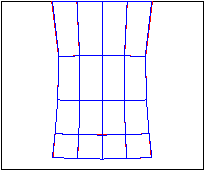
\includegraphics[width=.45\textwidth]{./graph/elasticity/stalactite-0}}
  \subfigure[{$\lambda = 10$}]{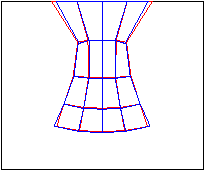
\includegraphics[width=.45\textwidth]{./graph/elasticity/stalactite-1}}
  \subfigure[{$\lambda = 100$}]{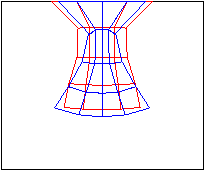
\includegraphics[width=.45\textwidth]{./graph/elasticity/stalactite-2}}
  \subfigure[{$\lambda = 1000$}]{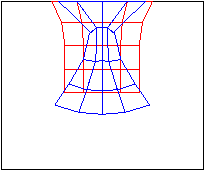
\includegraphics[width=.45\textwidth]{./graph/elasticity/stalactite-3}}
  \subfigure[{$\lambda = 10000$}]{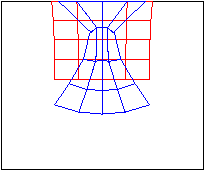
\includegraphics[width=.45\textwidth]{./graph/elasticity/stalactite-4}}
  \subfigure[{$\lambda = 100000$}]{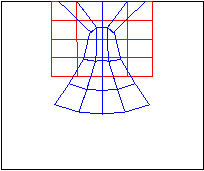
\includegraphics[width=.45\textwidth]{./graph/elasticity/stalactite-5}}
  \caption{Approximation with standard finite elements (red) and
    ``good'' elements (blue) for $\mu=1$ and different values of
    $\lambda$.}
  \label{fig:elasticity-compressibility}
\end{figure}

\begin{intro}
  As we could see in the preceding problem and example, approximation of the
  solution to the Lamé-Navier equations becomes difficult, if
  $\lambda \gg \mu$. In this case, the material is called almost
  incompressible, since the divergence measures compression or
  dilation and the dominating divergence term forces the divergence of
  the solution to be small. These cases are important in engineering
  and they initiated a lot of the research that resulted in the topics
  of this class.
\end{intro}

\begin{intro}
  A way to approach this problem is the introduction of an auxiliary variable
  \begin{gather*}
    p = -\lambda \div u.
  \end{gather*}
  Entering this definition into the Lamé-Navier equations, we obtain
  the following weak formulation.
\end{intro}

\begin{Definition}{displacement-pressure}
  The \define{displacement-pressure formulation} of the Lamé-Navier
  equations reads: find a pair $(u,p) \in V\times Q$ such that
  \begin{gather}
    \label{eq:lame-navier-mixed}
    \begin{aligned}
      2\mu\form(\strain u, \strain v) &- \form(p,\div v) &=&\form(f,v)
      &\forall v&\in V\\
      -\form(q,\div u) &-\tfrac1\lambda \form(p,q) &=&0
      &\forall q&\in Q.\\      
    \end{aligned}
  \end{gather}
  Equivalently, we write this in a single equation as
  \begin{multline}
    2\mu\form(\strain u, \strain v) - \form(p,\div v)
    - \form(q,\div u) -\tfrac1\lambda \form(p,q)
    = \form(f,v)
    \\
    \qquad\forall v\in V, q\in Q,
  \end{multline}
  or in the nonsymmetric, (semi-)definite version
  \begin{multline}
    2\mu\form(\strain u, \strain v) + \form(p,\div v)
    - \form(q,\div u) +\tfrac1\lambda \form(p,q)
    = \form(f,v)
    \\
    \qquad\forall v\in V, q\in Q,
  \end{multline}
  Here, $V$ is as before and $Q=L^2(\domain)$.
\end{Definition}

\begin{remark}
  The three forms have different purposes and will be used
  accordingly. The first one highlights the fact that we now have a
  system of equations, each equation tested with its own test
  function. The second and third stress the fact that we now have a
  bilinear form on the product space $X=V\times Q$.
  
  The second form is symmetric, but we will see later that is
  indefinite. Thus, non of our tools from functional analysis
  apply. In contrast, the third form is nonsymmetric, but we have
  \begin{multline*}
    2\mu\form(\strain u, \strain u) + \form(p,\div u)
    - \form(p,\div u) +\tfrac1\lambda \form(p,p)
    \\
    = 2\mu\form(\strain u, \strain u) + \tfrac1\lambda \form(p,p)
    \ge \tfrac{2\mu}{c_K} \norm{u}_{H^1}^2 + \tfrac1\lambda \form(p,p).
  \end{multline*}
  Thus, we have ellipticity with respect to the norm
  \begin{gather}
    \norm{(u,p)}_X^2 = \norm{u}_{H^1}^2 + \norm{p}_{L^2}^2.
  \end{gather}
  Nevertheless, the ellipticity constant depends on $\lambda$, and for
  large $\lambda$, we loose sharpness of estimates again.
\end{remark}

\begin{Definition}{lame-navier-strong}
  Integrating the first equation by parts, we
  obtain the \textbf{strong form} of the Lamé-Navier equations
  \begin{gather}
    \arraycolsep.2ex
    \begin{matrix}
      2\mu \div \strain u &+& \nabla p &=& f \\
      \div u &+& \tfrac1\lambda p &=& 0
    \end{matrix}
  \end{gather}
\end{Definition}

\section{Abstract saddle-point systems}
%\subsection{Notation and basic properties}

\begin{intro}
  In order to study the mathematics not only of the Lamé-Navier
  equations but of more general systems of the form of
  equation~\eqref{eq:lame-navier-mixed}, we introduce abstract
  bilinear forms
  \begin{gather}
    \label{eq:mixedintro:1}
    \begin{aligned}
      a(u,v) &= 2\mu\form(\strain u, \strain u), &u,v&\in V \\
      b(u,p) &=  -\form(p,\div u), & u&\in V, p\in Q\\
      c(p,q) &= \tfrac1\lambda \form(p,q) & p,q&\in Q.
    \end{aligned}
  \end{gather}
\end{intro}

\begin{Definition}{saddle-point-operators}
  For each of the bilinear forms, we define associated operators
  \begin{gather}
    \begin{aligned}
      A&\colon V \to V^* & \scal(Au,v) &= a(u,v), \\
      B&\colon V \to Q^* & \scal(Bu,q) &= b(u,q), \\
      B^T&\colon Q \to V^* & \scal(B^T p,v) &= b(v,p), \\
      C&\colon Q\to Q^* & \scal(C p,q) &= c(p,q).
    \end{aligned}
  \end{gather}
  Here, $\scal(.,.)$ is the canonical pairing between an element of
  the dual space and the space itself.
\end{Definition}

\begin{Definition}{saddle-point-abstract}
  The abstract saddle-point problem in weak form reads: find a pair
  $(u,p)\in V\times Q$ such that
  \begin{gather}
    \label{eq:saddle-point-weak}
    \arraycolsep.1em
    \begin{matrix}
      a(u,v) &+& b(v,p) &=& f(v) &\quad&\forall v\in V, \\
      b(u,q) &-& c(p,q) &=& g(q) &&\forall q\in Q.
    \end{matrix}
  \end{gather}
  In operator notation, it reads
  \begin{gather}
    \label{eq:saddle-point-operator}
    \arraycolsep.1em
    \begin{matrix}
      Au &+& B^T p &=& f &\quad&\text{in } V^*, \\
      Bu &-& C p &=& g &&\text{in } Q^*.
    \end{matrix}
  \end{gather}  
\end{Definition}

\begin{Notation}{saddle-point-form}
  In order to consider the whole bilinear form of the saddle-point
  system on the space $X = V\times Q$, we introduce
  \begin{gather}
    \mathcal A\mixedform(u,p,v,q)
      = a(u,v) + b(v,p) + b(u,q) - c(p,q)
  \end{gather}
\end{Notation}

\begin{Definition}{schur-complement}
  Let the operator $A:V\to V^*$ in the saddle-point system be
  invertible. Then, we define the \define{Schur complement} operator
  $S\colon Q\to Q^*$ of the system as
  \begin{gather}
      S= -B A^{-1} B^T - C.
  \end{gather}
\end{Definition}

\begin{Lemma}{schur-complement1}
  Formally, the saddle-point system~\eqref{eq:saddle-point-operator}
  can be solved in two steps by solving
  \begin{align}
    S p &= g - B A^{-1} f,\\
    A u &= f-B^T p.
  \end{align}
\end{Lemma}

\begin{proof}
  Formally solve the first equation
  of~\eqref{eq:saddle-point-operator} for $u$ and enter into the
  second.
\end{proof}

\begin{Lemma}{schur-definiteness}
  Let $a(.,.)$ be elliptic and $c(.,.)$ be positive semi-definite, and
  let $b(.,.)$ not be the zero form. Then, the bilinear form
  $\mathcal A(.,.)$ is indefinite.
\end{Lemma}

\begin{proof}
  First, we note that because of ellipticity of $a(.,.)$
  \begin{gather*}
    \mathcal A\mixedform(u,0,u,0) = a(u,u) \ge \gamma \norm{u}_V^2,
  \end{gather*}
  for some positive constant $\gamma$. Furthermore, $A$ is invertible
  and its inverse is positive definite. Furthermore,
  $A^{-1}B^T\colon Q\to V$. Then, choosing $v=-A^{-1}B^T p$ yields
  \begin{align*}
    \mathcal A\mixedform(v,p,v,p)
    &= a(A^{-1}B^T p,A^{-1}B^T p) - 2b(A^{-1}B^T p,p) - c(p,p) \\
    &= \scal(B^T p,A^{-1}B^T p) - 2\scal(A^{-1}B^T p,B^T p) - c(p,p)\\
    &= -\scal(B^T p,A^{-1}B^T p) - c(p,p).
  \end{align*}
  The first term is a quadratic term with the bilinear form associated
  with $A^{-T}$, which is positive definite. Since $b(.,.)$ is not the
  zero form, there is some $p$ such that $v\neq 0$. Therefore, with
  the minus sign and the semi-definiteness of $c(.,.)$ we have found a
  vector such that
  \begin{gather*}
    \mathcal A\mixedform(v,p,v,p) < 0.
  \end{gather*}
\end{proof}

\begin{remark}
  The previous result holds in particular for $c(.,.) \equiv 0$.
\end{remark}

%%%%%%%%%%%%%%%%%%%%%%%%%%%%%%%%%%%%%%%%%%%%%%%%%%%%%%%%%%%%%%%%%%%%%%
%%%%%%%%%%%%%%%%%%%%%%%%%%%%%%%%%%%%%%%%%%%%%%%%%%%%%%%%%%%%%%%%%%%%%%
\section{Stokes equations}

\begin{intro}
  When we write the Lamé-Navier equations in mixed form according to
  Definition~\ref{Definition:displacement-pressure}, there is no
  parameter $\lambda$ tending to infinity when the material becomes
  more and more compressible. Instead, there is the parameter
  $1/\lambda$ tending to zero. Thus, we can simply consider the case
  of incompressible material by setting $1/\lambda=0$ or, in our
  abstract framework~\eqref{eq:mixedintro:1} setting $c(.,.) = 0$. The
  resulting system is not only important for incompressible
  elasticity, but also models the slow flow of a very viscous liquid,
  so called \putindex{creeping flow}.
\end{intro}

\begin{Definition}{stokes-eq1}
  The \define{Stokes equations} in strong form are
    \begin{gather}
      \label{eq:mixedintro:stokes-strong1}
      \arraycolsep.2ex
      \begin{matrix}
        2\mu \div \strain u &+& \nabla p &=& f \\
        \div u && &=& 0.
      \end{matrix}
    \end{gather}
    In weak form, they are: find $u\in V \subset H^1(\domain;\R^d)$
    and $p\in Q \subset L^2(\domain)$ such that
  \begin{gather}
    \label{eq:mixedintro:stokes-weak1}
    \begin{aligned}
      2\mu\form(\strain u, \strain v) &- \form(\div v,p) &=&\form(f,v)
      + \text{bdry}
      &\forall v&\in V\\
      -\form(\div u,q) & &=&0+ \text{bdry}
      &\forall q&\in Q.\\      
    \end{aligned}
  \end{gather}
  The subspaces $V$ and $Q$ are determined by boundary conditions.
\end{Definition}

\begin{Definition}{solenoidal}
  A vector-valued function $u$ is called \define{divergence-free} or
  \define{solenoidal}, if there holds
  \begin{gather*}
    \div u = 0.
  \end{gather*}
  Flow described by a solenoidal function is called
  \define{incompressible}.
\end{Definition}

\begin{Lemma}{stokes-equivalence}
  Let $V=H^1_0(\domain;\R^d)$. Then, for any solenoidal function $u\in
  V$ there holds
  \begin{gather}
    \label{eq:mixedintro:6}
    2\mu\form(\strain u, \strain v) = \mu\form(\nabla u, \nabla v)
    \qquad\forall v\in V.
  \end{gather}
\end{Lemma}

\begin{proof}
  We have
  \begin{align*}
    \strain u: \strain v &= \sum_{i}^d \left[
    \d_i u_i\d_i v_i
    + \frac14\sum_{j\neq i} (\d_i u_j+\d_j u_i) (\d_i v_j+\d_j v_i)
    \right]
    \\
    &= \frac12\sum_{i,j=1}^d \d_i u_j\d_iv_j
    + \frac12\sum_{i=1}^d \d_i u_i \d_iv_i
    + \frac12\sum_{\substack{i,j=1\\j\neq i}}^d \d_i u_j\d_j v_i.
  \end{align*}
  The first term is the desired result, thus we have to eliminate the
  other two. We integrate by parts to obtain
  \begin{align*}
    \int_\domain \sum_{j\neq i} \d_i u_j\d_j v_i \dx
    &= - \int_\domain \sum_{j\neq i} \d_{ij}u_j v_i \dx\\
    &= \int_\domain \d_{ii} u_i v_i \dx \\
    &= -\int_\domain \d_i u_i \d_i v_i,
  \end{align*}
  where the second equality is due to $\div u=0$. Entering in the
  previous equation, we obtain
  \begin{gather*}
    \int_\domain \strain u:\strain v\dx
    = \int_\domain \nabla u:\nabla v\dx.
  \end{gather*}
\end{proof}

\begin{intro}
  In order to simplify subsequent discussion, it is customary to use
  the previous lemma to simplify the Stokes equations and to replace
  the strain tensor by the gradient. As a result, we can avoid the use
  of a Korn inequality and operate directly with the inner product of
  $H^1$. We note though that this formulation, while mathematically
  simpler, is physically wrong if $u\neq H^1_0(\domain;\R^d)$.
\end{intro}

\begin{Definition}{stokes-eq2}
  The simplified \define{Stokes equations} in strong form are
    \begin{gather}
      \label{eq:mixedintro:stokes-strong2}
      \arraycolsep.2ex
      \begin{matrix}
        \nu \Delta u &+& \nabla p &=& f \\
        \div u && &=& 0.
      \end{matrix}
    \end{gather}
    In weak form, they are: find $u\in V \subset H^1(\domain;\R^d)$
    and $p\in Q \subset L^2(\domain)$ such that
  \begin{gather}
    \label{eq:mixedintro:stokes-weak2}
    \begin{aligned}
      2\mu\form(\nabla u, \nabla v) &- \form(\div v,p) &=&\form(f,v)
      + \text{bdry}
      &\forall v&\in V\\
      -\form(\div u,q) & &=&0+ \text{bdry}
      &\forall q&\in Q.\\      
    \end{aligned}
  \end{gather}
  The subspaces $V$ and $Q$ are determined by boundary conditions.
\end{Definition}

\begin{Definition}{stokes-boundary2}
  Typical boundary conditions for the Stokes problem are
  \begin{xalignat}3
    \text{no-slip:}&& u &= 0,\\
    \text{free:}&& \d_n u + p n &= 0 ,\\
    \text{slip:}&& u_n &= 0 & \d_n u_\tau = 0,\\
    \text{friction:}&& u_n &= 0 & \d_n u_\tau = \alpha u_\tau.
  \end{xalignat}
  Here, $u_n$ and $u_\tau$ are the normal and tangential components of
  $u$ at the boundary.
\end{Definition}

\begin{remark}
  Very much the same way as for elliptic equations, boundary
  conditions on the function $u$ itself are essential boundary
  conditions which have to be incorporated into the space $V$, while
  those on the normal derivatives are the result of integration by
  parts and thus of the type of natural boundary conditions.

  All of the conditions above can also be imposed with nonzero data,
  where the physical meaning of such a condition might be debatable in
  some cases. Mathematically, inhomogeneous essential boundary
  conditions are achieved by lifting an arbitrary function with this
  boundary condition and modifying the right hand side of the
  equation, while inhomogeneous conditions on the normal derivative
  are implemented by boundary integrals on the right hand side.
\end{remark}

\begin{remark}
  Physically, the condition $u_n=0$ models an impermeable wall. It
  says in particular, that no mass is lost through this boundary and
  is thus related to the first principle of mass conservation.

  The conditions on the tangential velocity model the fact that
  molecules very close to the wall stick to the wall. While this claim
  is not supported by a frist principle, it has been verified by
  measurements to very high accuracy. Nevertheless, in the study of
  turbulent flow, a friction condition comes up quite naturally.
\end{remark}

\begin{Lemma}{divergence-compatibility}
  For any solenoidal $u$ function there holds
  \begin{gather}
    \int_{\d\domain} u\cdot n\ds = 0.
  \end{gather}
  Furthermore, if the boundary condition $u_n=0$ holds on the whole
  boundary $\d\domain$, then the pressure $p$ is determined by the
  Stokes equations only up to a constant.
\end{Lemma}

\begin{proof}
  The first statement is simple application of the Gauss theorem
  \begin{gather*}
    \int_{\domain} \div u\dx = \int_{\d\domain} u\cdot n\ds.
  \end{gather*}
  For the second statement, we note that the only term in the
  equations which determines the pressure is $\form(\div v,
  p)$. Integrating by parts and using the boundary condition, we
  obtain
  \begin{gather*}
    \int_\domain \div vp\dx = -\int_\domain v\nabla p\dx +
    \int_{\d\domain} v\cdot n p\ds = -\int_\domain v\nabla p\dx.
  \end{gather*}
  Since the gradient of a constant is zero, we can add any constant
  function to a given dolution $p$ without changing the term
  $\form(\div v,p)$, thus leaving $p$ determined only up to a
  constant.
\end{proof}

\begin{Notation}
  If in Definition~\ref{Definition:stokes-eq2} the space $V$ is chosen
  such that for all $v\in V$ there holds $v\cdot n =0$ on the whole
  boundary $\d\domain$, then the pressure solution $p$ cannot be
  determined uniquely in $L^2(\domain)$. In such cases, we chose the
  pressure space
  \begin{gather}
    L^2_0(\domain) = L^2(\domain)/\R
    = \biggl\{q\in L^2(\domain)\bigg| \int_\domain q\dx = 0\bigg\}. 
  \end{gather}
\end{Notation}

\begin{remark}
  As we could see from the preceding lemma, solvability of
  equation~\eqref{eq:mixedintro:stokes-weak2} depends on some
  compatibility of the spaces $V$ and $Q$ we had not seen in the
  elliptic case. Indeed, we need a whole new tool from functional
  analysis to replace the Lax-Milgram lemma. This tool will be studied
  in Chapter~\ref{sec:welposedness}.
\end{remark}

%%% Local Variables: 
%%% mode: latex
%%% TeX-master: "main"
%%% End: 
